% =============================================================================
%  Price Tag Vision — Лента Tech Life Hack 2026
%  Engine:  xelatex      (Unicode + системные шрифты)
%  Build:   xelatex -interaction=nonstopmode presentation.tex  (2 раза)
% =============================================================================
\documentclass[aspectratio=169,10pt]{beamer}

\usepackage{fontspec}
\usepackage{tikz}
\usepackage{xcolor}
\usepackage{booktabs}
\usepackage{array}
\usepackage{ragged2e}
\usepackage{graphicx}
\usepackage{hyperref}
\usetikzlibrary{arrows.meta,calc,fit,positioning,shapes.geometric,backgrounds,decorations.pathreplacing}

\setsansfont{PT Sans}
\setmonofont{JetBrains Mono}[Scale=0.82,Ligatures=NoCommon]
\renewcommand{\familydefault}{\sfdefault}

\definecolor{ink}{HTML}{0F172A}
\definecolor{slate}{HTML}{1E293B}
\definecolor{muted}{HTML}{64748B}
\definecolor{line}{HTML}{CBD5E1}
\definecolor{panel}{HTML}{F1F5F9}
\definecolor{bg}{HTML}{FFFFFF}
\definecolor{accent}{HTML}{2563EB}
\definecolor{accentTwo}{HTML}{0EA5E9}
\definecolor{good}{HTML}{059669}
\definecolor{warn}{HTML}{D97706}
\definecolor{redtag}{HTML}{DC2626}
\definecolor{violet}{HTML}{7C3AED}
\definecolor{dark}{HTML}{0B1220}

\hypersetup{colorlinks=true,linkcolor=accent,urlcolor=accent}

\setbeamertemplate{navigation symbols}{}
\setbeamercolor{normal text}{fg=ink,bg=bg}
\setbeamercolor{frametitle}{fg=ink,bg=bg}
\setbeamercolor{title}{fg=ink}
\setbeamercolor{block title}{fg=ink,bg=panel}
\setbeamercolor{block body}{fg=ink,bg=panel}
\setbeamercolor{structure}{fg=accent}
\setbeamercolor{itemize item}{fg=accent}
\setbeamercolor{itemize subitem}{fg=accentTwo}
\setbeamerfont{frametitle}{size=\large,series=\bfseries}
\setbeamerfont{block title}{size=\footnotesize,series=\bfseries}
\setbeamerfont{block body}{size=\footnotesize}
\setbeamertemplate{blocks}[rounded][shadow=false]
\setbeamertemplate{itemize item}{\raisebox{0.18ex}{\tiny$\blacksquare$}}
\setbeamertemplate{itemize subitem}{\raisebox{0.18ex}{\tiny$\bullet$}}

\setbeamertemplate{frametitle}{%
  \vspace{0.55em}%
  \begin{minipage}{\dimexpr\paperwidth-2em\relax}%
    \raggedright\color{ink}\large\bfseries\insertframetitle\par
    \vspace{0.15em}%
    \textcolor{accent}{\rule{1.4em}{1.6pt}}%
  \end{minipage}%
  \vspace{0.15em}%
}

\setbeamertemplate{footline}{%
  \leavevmode\hbox{%
    \begin{beamercolorbox}[wd=\paperwidth,ht=2.4ex,dp=1ex,leftskip=1.2em,rightskip=1.2em]{normal text}%
      \scriptsize\color{muted}%
      Price Tag Vision~$\cdot$~Team Козырный Бутерброд\hfill
      \insertframenumber\,/\,\inserttotalframenumber%
    \end{beamercolorbox}%
  }%
}

\newcommand{\code}[1]{{\ttfamily\small\color{slate}#1}}
\newcommand{\dashdash}{\symbol{"2D}\symbol{"2D}}
\newcommand{\hl}[1]{{\bfseries\color{accent}#1}}
\newcommand{\hr}[1]{{\bfseries\color{redtag}#1}}
\newcommand{\hg}[1]{{\bfseries\color{good}#1}}
\newcommand{\pill}[2]{%
  \tikz[baseline=-0.55ex]\node[rounded corners=2pt,draw=#1,fill=#1!10,
        inner xsep=4pt,inner ysep=1.5pt,line width=0.4pt,
        font=\scriptsize\bfseries,text=#1]{\strut #2};%
}
\newcommand{\smalltitle}[1]{{\small\bfseries\color{ink}#1}}

\tikzset{
  box/.style={rounded corners=3pt,draw=line,fill=white,line width=0.5pt,
              inner sep=4pt,align=center,text=ink,font=\scriptsize},
  techbox/.style={box,minimum width=2.55cm,minimum height=0.95cm},
  modelbox/.style={techbox,draw=accent!50,fill=accent!8,text=accent},
  storebox/.style={techbox,draw=accentTwo!50,fill=accentTwo!8,text=accentTwo!75!black},
  goodbox/.style={techbox,draw=good!50,fill=good!10,text=good},
  violetbox/.style={techbox,draw=violet!50,fill=violet!10,text=violet},
  dataflow/.style={-{Latex[length=2.2mm]},line width=0.7pt,draw=slate},
  softflow/.style={-{Latex[length=2.0mm]},line width=0.5pt,draw=muted!75,densely dashed},
  lane/.style={rounded corners=5pt,draw=line,fill=panel!60,inner sep=7pt}
}

\title{Price Tag Vision}
\author{Team Козырный Бутерброд}
\date{Лента Tech Life Hack 2026}

\begin{document}

% ===== Слайд 1 — Титул =======================================================
{\setbeamertemplate{footline}{}
\begin{frame}[plain]
  \begin{tikzpicture}[remember picture,overlay]
    \fill[dark] (current page.south west) rectangle (current page.north east);
    \fill[accent] (current page.south west) rectangle
      ($(current page.south west)+(0.20\paperwidth,0.13\paperheight)$);
    \fill[accentTwo] ($(current page.south west)+(0.20\paperwidth,0)$) rectangle
      ($(current page.south west)+(0.34\paperwidth,0.13\paperheight)$);
    \fill[violet] ($(current page.south west)+(0.34\paperwidth,0)$) rectangle
      ($(current page.south west)+(0.42\paperwidth,0.13\paperheight)$);
    \node[anchor=north east,align=right,text=white!85] at
      ($(current page.north east)+(-0.7,-0.65)$)
      {\small\bfseries Team Козырный Бутерброд\\[-0.15em]
       \scriptsize\color{white!55} Лента Tech Life Hack 2026};
    \begin{scope}[shift={($(current page.east)+(-1.6,-0.4)$)}]
      \foreach \i/\h in {0/0.5,1/0.7,2/0.95,3/1.25,4/1.05}{
        \fill[accent!\the\numexpr80-\i*12\relax,opacity=0.92]
          (\i*0.4,0) rectangle ++(0.28,\h);}
      \draw[accentTwo,line width=0.7pt,-{Stealth[length=3pt]}]
        (-0.3,0.18) -- (2.3,0.18);
    \end{scope}
    \node[anchor=west,text=white] at ($(current page.west)+(0.85,1.05)$)
      {\fontsize{34}{37}\selectfont\bfseries Price Tag Vision};
    \node[anchor=west,text width=0.78\paperwidth,text=white!82] at
      ($(current page.west)+(0.88,0.05)$)
      {\Large AI-пайплайн извлечения ценников\\[0.05em] из видео полок робота};
    \node[anchor=west,text=white!72] at ($(current page.west)+(0.88,-1.1)$)
      {\footnotesize
       \pill{accentTwo}{YOLOv8m + ByteTrack}\hspace{0.4em}};
  \end{tikzpicture}
\end{frame}}

% ===== Слайд 2 — Команда =====================================================
\begin{frame}{Команда}
  \vspace{0.25em}
  \begin{columns}[T,onlytextwidth]
    \begin{column}{0.24\textwidth}
      \begin{block}{Мирасов Константин}
        \footnotesize ML / CV инженер\\[0.35em]
        \scriptsize YOLOv8m, ByteTrack, обучение детектора\\[0.35em]
        \tiny\color{accent}\code{tg: @mezgou237}
      \end{block}
    \end{column}
    \begin{column}{0.24\textwidth}
      \begin{block}{Щербухина Анастасия}
        \footnotesize OCR / каталог\\[0.35em]
        \scriptsize PaddleOCR, \code{db\_hack.csv}, резолвер\\[0.35em]
        \tiny\color{accent}\code{tg: @anana7yk}
      \end{block}
    \end{column}
    \begin{column}{0.24\textwidth}
      \begin{block}{Сидимеков Дмитрий}
        \footnotesize Бэкенд-инженер\\[0.35em]
        \scriptsize FastAPI, Redis/RQ, MinIO\\[0.35em]
        \tiny\color{accent}\code{tg: @dimon8582}
      \end{block}
    \end{column}
    \begin{column}{0.24\textwidth}
      \begin{block}{Заплатин Артур}
        \footnotesize Фронтенд-инженер\\[0.35em]
        \scriptsize React, Vite, TypeScript\\[0.35em]
        \tiny\color{accent}\code{tg: @ArturZaplatin}
      \end{block}
    \end{column}
  \end{columns}
  \vspace{0.65em}
  \begin{block}{Главный вывод проекта (без приукрашивания)}
    \footnotesize На предоставленном дальнем 4K-видео целевой контест-скор
    \hr{физически недостижим} (доказано тремя способами). Мы построили
    честный, измеримый, разворачиваемый продукт и \hl{максимизировали то,
    что реально извлекаемо}.
  \end{block}
\end{frame}

% ===== Слайд 3 — Задача и бизнес-ценность ====================================
\begin{frame}{Задача и бизнес-ценность}
  \begin{columns}[T,onlytextwidth]
    \begin{column}{0.55\textwidth}
      \smalltitle{Что на самом деле требуется}\vspace{0.35em}
      \begin{itemize}\setlength\itemsep{2pt}
        \item Робот движется вдоль полок и снимает 4K-видео.
        \item Задача — превратить это видео в \hl{структурированный CSV}, где \hl{одна строка = один уникальный ценник}.
        \item Это \hl{видео $\to$ структурированные данные}, а не <<распознай картинку>>.
        \item Цель данных — мониторинг полок, аудит цен и аналитика ассортимента.
      \end{itemize}
      \vspace{0.7em}
      \begin{block}{Критерий контеста}
        \footnotesize Строка зачтена, если \hl{$\geq$80\% непустых GT-полей} совпали.
        Ключ сопоставления — штрихкод; иначе геометрия (IoU\,$\geq$\,0.5).
      \end{block}
    \end{column}
    \begin{column}{0.40\textwidth}
      \vspace{0.4em}
      \begin{tikzpicture}[node distance=0.45cm]
        \node[modelbox,minimum width=5.3cm,minimum height=0.85cm,font=\small\bfseries] (v) {Видео полок робота\\[-0.1em]\scriptsize\mdseries 4K MP4, движущаяся камера};
        \node[techbox,below=of v,minimum width=5.3cm,minimum height=0.85cm,draw=accent!55,fill=accent!8,text=accent,font=\small\bfseries] (p) {CV/OCR пайплайн\\[-0.1em]\scriptsize\mdseries detect $\to$ track $\to$ read $\to$ resolve};
        \node[goodbox,below=of p,minimum width=5.3cm,minimum height=0.85cm,font=\small\bfseries] (c) {Структурированный CSV\\[-0.1em]\scriptsize\mdseries 29 колонок, 1 строка = 1 ценник};
        \draw[dataflow] (v)--(p); \draw[dataflow] (p)--(c);
      \end{tikzpicture}
      \vspace{0.55em}
      \begin{block}{Бизнес-ценность}
        \begin{itemize}\setlength\itemsep{1pt}
          \item Быстрый аудит выкладки и цен.
          \item Снижение ручной разметки.
          \item Связь ценника с каталогом товаров.
        \end{itemize}
      \end{block}
    \end{column}
  \end{columns}
\end{frame}

% ===== Слайд 4 — Входные данные ==============================================
\begin{frame}{Входные данные: реальные видео, реальный шум}
  \begin{columns}[T,onlytextwidth]
    \begin{column}{0.52\textwidth}
      \smalltitle{Что внутри датасета}\vspace{0.3em}
      \begin{itemize}\setlength\itemsep{1pt}
        \item Источник — \hl{видео робота} в реальной торговой точке.
        \item Кадр \hl{3840$\times$2160}; ценник занимает малую область.
        \item Есть размеченные и неразмеченные клипы.
        \item Один ценник виден в \hl{нескольких кадрах}.
      \end{itemize}
      \vspace{0.4em}
      \smalltitle{Почему сложно}\vspace{0.25em}
      \footnotesize
      \begin{itemize}\setlength\itemsep{0pt}
        \item \hr{блики} на пластике ценодержателей,
        \item \hr{размытие} из-за движения,
        \item \hr{перспектива} вдоль стеллажа,
        \item \hr{дальняя дистанция}: мелкий шрифт $\sim$10\,px.
      \end{itemize}
    \end{column}
    \begin{column}{0.44\textwidth}
      \vspace{0.2em}
      \begin{tikzpicture}[x=1cm,y=1cm]
        \def\W{6.0}\def\H{3.4}
        \node[draw=line,fill=panel,rounded corners=4pt,
              minimum width=\W cm,minimum height=\H cm,inner sep=0] at (\W/2,\H/2) {};
        \foreach \y in {0.5,1.5,2.5}{\draw[line] (0.1,\y) -- (\W-0.1,\y);}
        \foreach \x/\y in {0.5/0.85,1.1/0.9,1.7/0.85,2.4/0.92,3.0/0.85,3.7/0.9,4.3/0.88,4.9/0.92,5.4/0.88,0.55/1.85,1.15/1.88,1.75/1.85,2.45/1.9,3.1/1.85,3.75/1.88,4.4/1.85,5.0/1.9,0.6/2.85,1.2/2.82,1.85/2.85,2.55/2.88,3.25/2.85,3.95/2.88,4.6/2.85,5.2/2.88}{
          \fill[redtag!70] (\x,\y) rectangle ++(0.20,0.14);}
        \fill[white,opacity=0.55] (3.2,0.6) ellipse (1.2 and 0.45);
        \draw[accent,line width=0.9pt] (2.35,0.78) rectangle ++(0.27,0.21);
        \node[font=\tiny\bfseries\color{accent},anchor=west] at (2.67,0.88) {bbox};
        \node[anchor=north west,font=\tiny\bfseries\color{muted}] at (0.05,\H-0.05) {ВИД ПОЛКИ $\cdot$ 4K $\cdot$ движение робота};
      \end{tikzpicture}
      \vspace{0.35em}
      \begin{block}{Следствие}
        Один ценник \hl{в N кадрах} $\Rightarrow$ нужны \hl{трекинг и дедупликация}, чтобы не множить строки CSV.
      \end{block}
    \end{column}
  \end{columns}
\end{frame}

% ===== Слайд 5 — Архитектура ==================================================
\begin{frame}{Сквозная архитектура продукта}
  \vspace{-0.4em}
  \centering
  \resizebox{0.96\textwidth}{!}{%
  \begin{tikzpicture}[node distance=0.7cm and 0.7cm]
    \node[techbox,fill=panel,minimum width=2.0cm] (user) {Пользователь\\\scriptsize браузер};
    \node[modelbox,right=of user,minimum width=2.55cm] (fe) {Фронтенд\\\scriptsize React + Vite + TS};
    \node[techbox,right=of fe,minimum width=2.55cm] (be) {API-бэкенд\\\scriptsize FastAPI};
    \node[storebox,above right=0.45cm and 0.85cm of be,minimum width=2.2cm] (pg) {PostgreSQL\\\scriptsize метаданные джобов};
    \node[storebox,below right=0.45cm and 0.85cm of be,minimum width=2.2cm] (rq) {Redis + RQ\\\scriptsize очередь задач};
    \node[techbox,right=0.9cm of be,xshift=2.5cm,minimum width=2.45cm] (wk) {Worker\\\scriptsize фоновое исполнение};
    \node[goodbox,right=of wk,minimum width=2.55cm] (vs) {Vision Service\\\scriptsize FastAPI + CV/OCR};
    \node[violetbox,below=1.35cm of wk,minimum width=2.55cm] (mi) {MinIO\\\scriptsize видео, CSV, артефакты};
    \draw[dataflow] (user)--(fe);
    \draw[dataflow] (fe)-- node[above,font=\tiny\color{muted}]{REST} (be);
    \draw[softflow] (be)--(pg); \draw[softflow] (be)--(rq);
    \draw[dataflow] (rq.east)-- node[above,sloped,font=\tiny\color{muted}]{dequeue} (wk.west);
    \draw[dataflow] (wk)-- node[above,font=\tiny\color{muted}]{HTTP} (vs);
    \draw[dataflow] (wk)--(mi);
    \draw[dataflow] (vs.south) -- ++(0,-0.45) -| (mi.east);
    \draw[softflow] (be.south) -- ++(0,-2.2) -| (mi.west);
    \begin{pgfonlayer}{background}
      \node[lane,fit=(fe)(be)(pg)(rq)(wk)(vs)(mi),
            label={[font=\tiny\bfseries\color{muted},anchor=north west]north west:ЛОКАЛЬНЫЙ КОНТУР $\cdot$ Docker Compose}] {};
    \end{pgfonlayer}
  \end{tikzpicture}}
  \vspace{0.4em}
  \begin{columns}[T,onlytextwidth]
    \begin{column}{0.52\textwidth}\footnotesize \hl{Сценарий.}\; Загрузка MP4 $\to$ создание джоба $\to$ опрос статуса $\to$ \hl{превью CSV} $\to$ скачивание CSV. Лимит времени на джоб \hl{снят} — длинное видео обрабатывается полностью.\end{column}
    \begin{column}{0.46\textwidth}\footnotesize \hl{Почему важно.}\; Продуктовый контур уже рабочий и демонстрируемый — модели улучшаются \emph{без} переписывания платформы (stateless vision-сервис).\end{column}
  \end{columns}
\end{frame}

% ===== Слайд 6 — CV-пайплайн v5 ==============================================
\begin{frame}{CV-пайплайн \code{price\_tag\_v5}: финальная версия}
  \vspace{-0.2em}\centering
  \begin{tikzpicture}[node distance=0.30cm and 0.30cm,
        stage/.style={box,minimum width=1.95cm,minimum height=1.05cm,align=center,font=\scriptsize}]
    \node[stage,fill=accent!8,draw=accent!50,text=accent] (in) {\bfseries MP4 4K\\ \mdseries робот};
    \node[stage,right=of in] (norm) {\bfseries Нормализация\\ \mdseries undistort+upright};
    \node[stage,right=of norm,fill=accent!8,draw=accent!50,text=accent] (det) {\bfseries YOLOv8m\\ \mdseries детекция};
    \node[stage,right=of det,fill=accent!8,draw=accent!50,text=accent] (trk) {\bfseries ByteTrack\\ \mdseries трекинг};
    \node[stage,right=of trk] (top) {\bfseries Top-K\\ \mdseries кропы};
    \node[stage,below=0.95cm of top,fill=violet!10,draw=violet!50,text=violet] (slot) {\bfseries Slot-merge\\ \mdseries фрагм.\,$\to$\,слот};
    \node[stage,left=of slot] (ocr) {\bfseries OCR кропа\\ \mdseries цена, токены};
    \node[stage,left=of ocr,fill=violet!10,draw=violet!50,text=violet] (cat) {\bfseries Каталог\\ \mdseries \code{db\_hack}};
    \node[stage,left=of cat] (fus) {\bfseries Слияние\\ \mdseries QR$\leftrightarrow$visible};
    \node[stage,left=of fus] (gate) {\bfseries Recall-gate\\ \mdseries +confidence};
    \node[stage,left=of gate,fill=good!10,draw=good!50,text=good] (csv) {\bfseries CSV 29 кол.\\ \mdseries +side-car};
    \draw[dataflow] (in)--(norm); \draw[dataflow] (norm)--(det); \draw[dataflow] (det)--(trk); \draw[dataflow] (trk)--(top);
    \draw[dataflow] (top.south) -- ++(0,-0.4) -| (slot.north);
    \draw[dataflow] (slot)--(ocr); \draw[dataflow] (ocr)--(cat); \draw[dataflow] (cat)--(fus); \draw[dataflow] (fus)--(gate); \draw[dataflow] (gate)--(csv);
    \draw[decorate,decoration={brace,amplitude=4pt},slate,line width=0.5pt]
      ($(in.north west)+(0,0.15)$) -- ($(top.north east)+(0,0.15)$)
      node[midway,above=3pt,font=\tiny\bfseries\color{slate}]{ЛОКАЛИЗАЦИЯ (унаследована из v2, проверена)};
    \draw[decorate,decoration={brace,amplitude=4pt},violet,line width=0.5pt]
      ($(slot.south east)+(0,-0.15)$) -- ($(csv.south west)+(0,-0.15)$)
      node[midway,below=3pt,font=\tiny\bfseries\color{violet}]{ИДЕНТИФИКАЦИЯ И ЭКСПОРТ (где новизна v5)};
  \end{tikzpicture}
  \vspace{0.7em}
  \begin{columns}[T,onlytextwidth]
    \begin{column}{0.60\textwidth}\footnotesize \hl{Ключевая идея.} Сначала находим ценник, агрегируем наблюдения по \emph{физическому слоту}, читаем маленький кроп и \emph{сопоставляем с каталогом} — а не пытаемся «дочитать» 4K-кадр.\end{column}
    \begin{column}{0.37\textwidth}\scriptsize \pill{accent}{детекция $\to$ трек}\; \pill{violet}{каталог-якорь}\; \pill{good}{recall + confidence}\end{column}
  \end{columns}
\end{frame}

% ===== Слайд 7 — Эволюция пайплайнов =========================================
\begin{frame}{Эволюция пайплайнов: что пробовали и почему}
  \vspace{-0.1em}\centering
  \begin{tikzpicture}[node distance=0.42cm,
      v/.style={box,minimum width=2.15cm,minimum height=1.55cm,align=center,font=\scriptsize,text width=2.0cm}]
    \node[v,fill=panel] (v1) {\bfseries v1 (cpu)\\[-0.1em]\mdseries базовый каркас\\\color{muted}доказал платформу};
    \node[v,right=of v1,draw=accent!50,fill=accent!8,text=accent] (v2) {\bfseries v2\\[-0.1em]\mdseries детектор+\\ByteTrack+\\zonal OCR};
    \node[v,right=of v2] (v3) {\bfseries v3\\[-0.1em]\mdseries реконструкция\\полей};
    \node[v,right=of v3] (v4) {\bfseries v4\\[-0.1em]\mdseries назначение\\по каталогу};
    \node[v,right=of v4,draw=good!55,fill=good!10,text=good] (v5) {\bfseries v5 (финал)\\[-0.1em]\mdseries каталог-якорь\\+recall+conf.};
    \draw[dataflow] (v1)--(v2); \draw[dataflow] (v2)--(v3); \draw[dataflow] (v3)--(v4); \draw[dataflow] (v4)--(v5);
  \end{tikzpicture}
  \vspace{0.5em}
  \begin{columns}[T,onlytextwidth]
    \begin{column}{0.5\textwidth}
      \begin{block}{Почему каждый шаг сменялся}\footnotesize
        \begin{itemize}\setlength\itemsep{1pt}
          \item \hl{v2}: зонный OCR медленный и хрупкий на дальней съёмке; точный мелкий шрифт нечитаем.
          \item \hl{v3}: попытка реконструировать поля из частичных чтений — нестабильно без опоры.
          \item \hl{v4}: первая идея каталога как источника истины.
          \item \hl{v5}: каталог-якорь + slot-merge + recall-gate + confidence — \hg{precision-first}.
        \end{itemize}
      \end{block}
    \end{column}
    \begin{column}{0.48\textwidth}
      \begin{block}{Общий вывод всех итераций}\footnotesize
        Все подходы упёрлись в \hr{одну и ту же физическую стену}: на этой
        дистанции мелкий шрифт \emph{не существует} в сигнале. Менялся не
        результат по этим полям, а \hl{качество того, что извлекаемо}:
        чистота строк, точность идентификации, покрытие.
        \vspace{0.25em}\\ v2/v3/v4 сохранены как fallback — \emph{ничего не сломано}.
      \end{block}
    \end{column}
  \end{columns}
\end{frame}

% ===== Слайд 8 — Детектор и датасет ==========================================
\begin{frame}{Детектор и датасет (как обучали YOLO)}
  \begin{columns}[T,onlytextwidth]
    \begin{column}{0.46\textwidth}
      \begin{block}{Локальный YOLO-датасет}\footnotesize
        \setlength{\tabcolsep}{4pt}\renewcommand{\arraystretch}{1.05}
        \begin{tabular}{@{}lr@{}}\toprule
          \textbf{Параметр} & \textbf{Значение}\\ \midrule
          Задача             & однокласс. детекция\\
          Класс              & \code{price tag}\\
          Всего изображений  & 83 (train 66 / val 11 / test 6)\\
          Размеченных боксов & 909 ($\sim$11 на кадр)\\
          Разметка           & авто-лейблинг + NCC-пропагация\\
          Формат             & YOLO (TXT)\\ \bottomrule
        \end{tabular}
      \end{block}
      \vspace{0.4em}
      \begin{block}{Обучение}\footnotesize
        \setlength{\tabcolsep}{4pt}
        \begin{tabular}{@{}ll@{}}
          База & \code{yolov8m.pt}\\
          Эпох & 100 \quad Размер 640 \quad Batch 16\\
          Девайс & GPU 0\\
          Веса & \code{runs/.../weights/best.pt}\\
        \end{tabular}
      \end{block}
    \end{column}
    \begin{column}{0.50\textwidth}
      \begin{block}{Финальные метрики валидации}\vspace{0.1em}\footnotesize
        \setlength{\tabcolsep}{6pt}\renewcommand{\arraystretch}{1.15}
        \begin{tabular}{@{}llr@{}}\toprule
          \textbf{Метрика} & & \textbf{Значение}\\ \midrule
          Precision    & \pill{good}{P}             & \textbf{0.926}\\
          Recall       & \pill{warn}{R}             & \textbf{0.787}\\
          mAP@50       & \pill{accent}{mAP50}       & \textbf{0.830}\\
          mAP@50--95   & \pill{accentTwo}{mAP50-95} & \textbf{0.623}\\ \bottomrule
        \end{tabular}
        \vspace{0.35em}
        \footnotesize\color{slate} Пик при обучении: \hl{mAP@50 = 0.872} (эпоха 43).
      \end{block}
      \vspace{0.3em}
      \begin{center}
      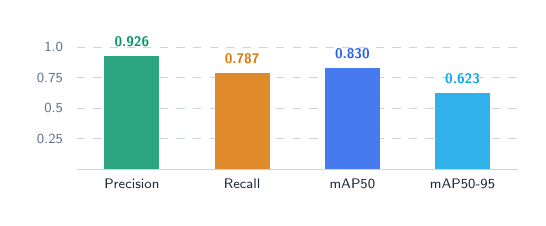
\begin{tikzpicture}[x=1cm,y=1.55cm]
        \draw[line] (0,0) -- (5.6,0);
        \foreach \v in {0.25,0.5,0.75,1.0}{\draw[line,dashed,line width=0.3pt] (0,\v) -- (5.6,\v); \node[anchor=east,font=\tiny\color{muted}] at (-0.05,\v) {\v};}
        \foreach \i/\v/\lbl/\col in {0/0.926/Precision/good,1/0.787/Recall/warn,2/0.830/mAP50/accent,3/0.623/mAP50-95/accentTwo}{
          \fill[\col!85] (\i*1.4+0.35,0) rectangle ++(0.7,\v);
          \node[anchor=south,font=\tiny\bfseries\color{\col}] at (\i*1.4+0.7,\v) {\v};
          \node[anchor=north,font=\tiny\color{slate}] at (\i*1.4+0.7,0) {\lbl};}
      \end{tikzpicture}
      \end{center}
      {\scriptsize\color{slate} Вывод: \hg{детекция — не узкое место}. Проблема — идентификация мелкого текста.}
    \end{column}
  \end{columns}
\end{frame}

% ===== Слайд 9 — Детекция и трекинг (реальный скриншот) ======================
\begin{frame}{Детекция и трекинг — 1 уникальный ценник = 1 строка}
  \begin{columns}[T,onlytextwidth]
    \begin{column}{0.40\textwidth}\vspace{0.1em}
      \begin{center}\fbox{\includegraphics[height=6.05cm,keepaspectratio]{assets/05_detection_tracking_showcase.jpg}}\end{center}
      \vspace{-0.3em}{\tiny\color{muted}\centering Кадр пайплайна: зелёные bbox + ID треков от YOLOv8m + ByteTrack.}
    \end{column}
    \begin{column}{0.58\textwidth}
      \begin{block}{Что показывает скриншот}\footnotesize
        \begin{itemize}\setlength\itemsep{2pt}
          \item YOLOv8m находит \hl{каждый ценник} — несмотря на блики, перспективу и плотность.
          \item ByteTrack связывает детекции в \hl{стабильный track ID}.
          \item \hl{Slot-merge} (v5) склеивает фрагменты ByteTrack одного физического ценника в один слот $\Rightarrow$ \hl{одна} строка CSV, даже если ценник снят 30 раз.
        \end{itemize}
      \end{block}
      \vspace{0.4em}
      \begin{block}{Проверено численно}\footnotesize
        Средний IoU сматченных строк \hg{0.67--0.69} — геометрия и
        bbox\,$\to$\,сырой кадр 3840$\times$2160 \hg{корректны} (доказано на
        строках, сматченных по штрихкоду, т.е.\ независимо от bbox).
      \end{block}
    \end{column}
  \end{columns}
\end{frame}

% ===== Слайд 10 — Распознавание (реальный скриншот) ==========================
\begin{frame}{Распознавание + резолвер по каталогу}
  \begin{columns}[T,onlytextwidth]
    \begin{column}{0.54\textwidth}\vspace{0.1em}
      \begin{center}\fbox{\includegraphics[width=0.88\linewidth,keepaspectratio]{assets/06_recognition_showcase.jpg}}\end{center}
      \vspace{-0.5em}{\scriptsize\color{muted} \textcolor{good}{\bfseries ACCEPTED}~--- каталог подтвердил; \textcolor{redtag}{\bfseries withheld}~--- precision-first отказ.}
    \end{column}
    \begin{column}{0.43\textwidth}
      \smalltitle{Что снимает кроп}\vspace{0.2em}
      \begin{itemize}\setlength\itemsep{1pt}\footnotesize
        \item \hl{Цены}: \code{price\_card}, \code{price\_default}, скидка.
        \item \hl{Бренд-токены} из верхней части ценника.
        \item \hl{QR} — когда декодируется (редко на дистанции).
      \end{itemize}
      \vspace{0.35em}
      \begin{block}{\code{db\_hack.csv} — каталог как опора}\footnotesize
        \setlength{\tabcolsep}{5pt}\renewcommand{\arraystretch}{1.0}
        \begin{tabular}{@{}lr@{}}\toprule
          Размер           & $\sim$50\,МБ\\
          Уникальных кодов & 355\,832\\
          Уникальных имён  & 136\,169\\
          Кодировка        & CP1251\\ \bottomrule
        \end{tabular}
      \end{block}
      \vspace{0.25em}
      {\scriptsize\color{slate} \hl{Идея.} Штрихкод не читается, но даже частичные латинские токены бренда матчат ценник в каталог. \hg{Точность имени на принятых = 100\%} — система \emph{никогда} не выдаёт неверный товар.}
    \end{column}
  \end{columns}
\end{frame}

% ===== Слайд 11 — UI и CSV ===================================================
\begin{frame}{Интерфейс и выходной артефакт}
  \begin{columns}[T,onlytextwidth]
    \begin{column}{0.50\textwidth}\vspace{0.1em}
      \begin{tikzpicture}[x=1cm,y=1cm]
        \def\W{7.0}\def\H{4.6}
        \fill[white,draw=line,rounded corners=4pt] (0,0) rectangle (\W,\H);
        \fill[panel,draw=line,rounded corners=4pt] (0,\H-0.55) rectangle (\W,\H);
        \foreach \cx/\col in {0.25/redtag,0.55/warn,0.85/good}{\fill[\col] (\cx,\H-0.28) circle (0.085);}
        \node[anchor=west,font=\tiny\color{muted}] at (1.2,\H-0.28) {http://localhost:5173 / Price Tag Vision};
        \fill[panel,draw=line,rounded corners=3pt] (0.3,0.35) rectangle (3.0,\H-0.95);
        \node[anchor=north west,font=\tiny\bfseries\color{ink}] at (0.42,\H-1.05) {ЗАГРУЗКА};
        \draw[accent,dashed,line width=0.5pt,rounded corners=3pt] (0.45,1.95) rectangle (2.85,3.30);
        \node[align=center,font=\tiny\color{accent}\bfseries] at (1.65,2.65) {Перетащите MP4\\или выберите};
        \fill[line] (0.45,1.45) rectangle (2.85,1.60);
        \fill[accent] (0.45,1.45) rectangle (2.10,1.60);
        \node[anchor=west,font=\tiny\color{slate}] at (0.45,1.30) {статус: \textbf{processing}};
        \node[anchor=west,font=\tiny\color{muted}] at (0.45,1.07) {этап = OCR / catalog $\cdot$ 68\%};
        \fill[accent,rounded corners=2pt] (0.45,0.50) rectangle (1.55,0.90);
        \node[font=\tiny\bfseries\color{white}] at (1.0,0.70) {Превью};
        \fill[good,rounded corners=2pt] (1.65,0.50) rectangle (2.85,0.90);
        \node[font=\tiny\bfseries\color{white}] at (2.25,0.70) {Скачать CSV};
        \node[anchor=north west,font=\tiny\bfseries\color{ink}] at (3.3,\H-1.05) {ПРЕВЬЮ СТРОК CSV};
        \fill[panel,draw=line,rounded corners=2pt] (3.25,1.55) rectangle (\W-0.25,\H-1.20);
        \foreach \y/\name/\p in {3.55/{POGGIO TOSCO}/1199.99,3.15/{LE VIGNE DI SAM.}/1015.00,2.75/{MINI MONTEP.}/1499.99,2.35/{CITRAN Бордо}/1899.99,1.95/{(withheld)}/--}{
          \node[anchor=west,font=\tiny\color{slate}] at (3.4,\y){\name};
          \node[anchor=east,font=\tiny\bfseries\color{ink}] at (\W-0.35,\y){\p};}
        \node[anchor=north west,font=\tiny\bfseries\color{ink}] at (3.3,1.45) {CONFIDENCE SIDE-CAR};
        \foreach \i/\c/\col in {0/high/good,1/med/warn,2/low/muted,3/low/muted,4/low/muted}{
          \fill[\col!75,rounded corners=1pt] (3.4+\i*0.72,0.50) rectangle ++(0.6,0.75);
          \node[font=\tiny\bfseries\color{white}] at (3.7+\i*0.72,0.88) {\c};}
      \end{tikzpicture}
    \end{column}
    \begin{column}{0.48\textwidth}
      \begin{block}{UX-поверхность (реализована)}\footnotesize
        \begin{itemize}\setlength\itemsep{1pt}
          \item Загрузка MP4 через drag-and-drop.
          \item Асинхронный джоб: статус, прогресс, этап.
          \item \hl{Живое превью строк CSV} (галерея кропов убрана — продукт — это таблица).
          \item \hl{Скачивание CSV} на 29 колонок.
        \end{itemize}
      \end{block}
      \vspace{0.3em}
      \begin{block}{Фрагмент реального CSV (схема: 29 колонок)}\scriptsize
        \setlength{\tabcolsep}{3pt}\renewcommand{\arraystretch}{1.05}
        \begin{tabular}{@{}p{2.55cm}rrl@{}}\toprule
          \tiny product\_name & \tiny card & \tiny disc & \tiny barcode\\ \midrule
          \tiny Вино CAHORS Шато Брю Лягардет     & \tiny 2105.99 & \tiny -7\% & \tiny 3661710013000\\
          \tiny Вино PREIGNES LE VIEUX Пэй дОк    & \tiny —       & \tiny —    & \tiny 3552848940002\\ \bottomrule
        \end{tabular}
        \vspace{0.2em}
        {\tiny\color{muted} bbox — в \hl{ориентации исходного видео} (доказано); рядом \code{debug/row\_confidence.json} — confidence/провенанс (high\,/\,medium\,/\,low).}
      \end{block}
    \end{column}
  \end{columns}
\end{frame}

% ===== Слайд 12 — Почему контест-скор физически = 0 ==========================
\begin{frame}{Почему контест-скор физически = 0 (доказано 3 раза)}
  \begin{columns}[T,onlytextwidth]
    \begin{column}{0.49\textwidth}
      \begin{block}{Реальность GT-полей (видео 26\_12-20, 71 строка)}\footnotesize
        \setlength{\tabcolsep}{5pt}\renewcommand{\arraystretch}{1.12}
        \begin{tabular}{@{}lr@{}}\toprule
          \textbf{Поле (мелкий шрифт)} & \textbf{Непусто в GT}\\ \midrule
          \code{id\_sku} (12 цифр)     & \hr{69 / 71}\\
          \code{code} (строка)         & \hr{61 / 71}\\
          \code{print\_datetime}       & \hr{45 / 71}\\ \midrule
          Среднее \#зачётных полей/стр & 21.4\\
          Мин.\ \#зачётных полей       & 15 (одна строка)\\ \bottomrule
        \end{tabular}
      \end{block}
      \vspace{0.3em}
      \begin{block}{Арифметика потолка}\footnotesize
        $\sim$7 нечитаемых полей/строку (\code{id\_sku}, \code{print\_datetime},
        \code{code}, копейки \code{price\_default}, \code{price1\_qr},
        \code{price2\_qr}, \code{special\_symbols}).\\[0.2em]
        Максимум $\approx$ \hr{15/22 $\approx$ 0.68} $<$ порог \hl{0.80}
        $\Rightarrow$ \hr{ни одна строка не зачитывается}.
      \end{block}
    \end{column}
    \begin{column}{0.49\textwidth}
      \begin{block}{Три независимых доказательства}\footnotesize
        \begin{itemize}\setlength\itemsep{2pt}
          \item[\textbf{1.}] Стандартный OCR, мульти-кроп пробы и
            \hl{визуальный декод штрихкода 0/14} — печатные штрихи
            суб-разрешимы на этой дистанции.
          \item[\textbf{2.}] \hl{Точная статистика GT}: $\geq$80\% порог
            требует $\sim$18/22, а $\sim$7 полей физически отсутствуют в
            сигнале (см.\ слева).
          \item[\textbf{3.}] \hl{Recall-анализ}: даже геометрически
            достижимо максимум \hr{48/71}, и каждая из этих строк всё равно
            $<$0.80 из-за мелкого шрифта.
        \end{itemize}
      \end{block}
      \vspace{0.2em}
      \begin{block}{Честный вывод}\footnotesize
        Это \hr{ограничение разрешения входных данных}, а не дефект
        пайплайна. Поэтому мы перестали гнаться за скором и стали
        максимизировать \hg{реально извлекаемое качество}.
      \end{block}
    \end{column}
  \end{columns}
\end{frame}

% ===== Слайд 13 — Что получилось / выводы ====================================
\begin{frame}{Что получилось, что нет и почему}
  \begin{columns}[T,onlytextwidth]
    \begin{column}{0.49\textwidth}
      \begin{block}{\textcolor{good}{Что получилось}}\footnotesize
        \begin{itemize}\setlength\itemsep{1.5pt}
          \item Детектор / трекинг / undistort / геометрия — \hg{корректны} (mean IoU 0.67--0.69).
          \item Каталог: \hg{точность имени 100\%} на принятых — никогда не выдаём неверный товар; штрихкод не подставляется при сомнении.
          \item \hl{Recall-gate}: покрытие GT \hg{19\,$\to$\,48 / 71}, сматчено \hg{14\,$\to$\,32} — при сохранённой точности.
          \item \hl{Confidence side-car} для триажа строк.
          \item Цены/скидки извлекаются; CSV в исходной ориентации.
          \item MVP: лимит времени джоба снят (docker\,=\,локаль), Docker-деплой, README на русском.
        \end{itemize}
      \end{block}
    \end{column}
    \begin{column}{0.49\textwidth}
      \begin{block}{\textcolor{redtag}{Что не получилось и почему}}\footnotesize
        \begin{itemize}\setlength\itemsep{1.5pt}
          \item \hr{barcode / SKU / date / code / копейки} — суб-Найквист на дальней 4K ($\sim$10\,px). \emph{Физика, не код.}
          \item \hr{Ослабление slot-merge} — измеренный тупик: \hr{48\,$\to$\,45}, без выигрыша. На движущейся камере слияние временных фрагментов размывает якорный bbox.
          \item \hr{Визуальный декод штрихкода 0/14}.
          \item \hr{Каталог \code{category="all"}} отклонён: точность имени 100\%\,$\to$\,80\%, $\times$27 медленнее. Неверная идентификация хуже пустой.
        \end{itemize}
      \end{block}
      \vspace{0.2em}
      {\scriptsize\color{slate} Принцип: \hl{precision-first}. Лучше честное «пусто/withheld», чем уверенная ошибка, которая ломает ключ сопоставления.}
    \end{column}
  \end{columns}
\end{frame}

% ===== Слайд 14 — Ограничения и масштабирование ==============================
\begin{frame}{Куда дальше и как масштабируется}
  \begin{columns}[T,onlytextwidth]
    \begin{column}{0.48\textwidth}
      \begin{block}{Реальные рычаги (всё упирается в разрешение)}\footnotesize
        \begin{itemize}\setlength\itemsep{1.5pt}
          \item \hl{Более близкая съёмка} или \hl{super-resolution} перед OCR — единственные пути к ненулевому скору.
          \item \hl{OCR зоны штрихкода} как подсказка цифр для выбора EAN-13 vs.\ GTIN-14.
          \item \hl{Мультикадровое накопление} токенов по всем кадрам слота.
          \item \hl{Авто-категория} каталога по визуальным признакам.
          \item Экспорт детектора в ONNX/TensorRT + батч-инференс.
        \end{itemize}
      \end{block}
    \end{column}
    \begin{column}{0.48\textwidth}
      \begin{block}{Масштабирование}\footnotesize
        \begin{itemize}\setlength\itemsep{1.5pt}
          \item \hl{Воркеры — горизонтально}: общая Redis-очередь, реплики \code{worker}\,/\,\code{vision-service}.
          \item Vision-сервис \hl{без состояния}: артефакты в S3/MinIO, по GPU на инстанс.
          \item Backend без состояния; Postgres/Redis — кластерные в проде.
          \item Узкое место — GPU vision-сервиса; очередь сглаживает пики.
        \end{itemize}
      \end{block}
      \vspace{0.25em}
      {\scriptsize\color{slate} \hl{Identity-слой улучшается без переписывания} продуктового контура — детектор, очередь, хранилище и UI остаются прежними.}
    \end{column}
  \end{columns}
\end{frame}

% ===== Слайд 15 — Прозрачность: модели, данные, железо =======================
\begin{frame}{Прозрачность: модели, данные, железо}
  \begin{columns}[T,onlytextwidth]
    \begin{column}{0.49\textwidth}
      \begin{block}{Модели и лицензии (всё локально, без облачных API)}\footnotesize
        \setlength{\tabcolsep}{4pt}\renewcommand{\arraystretch}{1.12}
        \begin{tabular}{@{}lll@{}}\toprule
          \textbf{Модель} & \textbf{Роль} & \textbf{Лицензия}\\ \midrule
          YOLOv8m (Ultralytics) & детектор   & \code{AGPL-3.0}\\
          PaddleOCR             & OCR        & \code{Apache-2.0}\\
          Tesseract (fallback)  & OCR rus+en & \code{Apache-2.0}\\
          ByteTrack             & трекинг    & \code{MIT}\\ \bottomrule
        \end{tabular}
        \vspace{0.25em}
        {\scriptsize\color{slate} Веса детектора обучены нами и лежат в репо (\code{best.pt}).}
      \end{block}
      \vspace{0.35em}
      \begin{block}{Данные и разметка (честно)}\footnotesize
        \begin{itemize}\setlength\itemsep{1pt}
          \item \code{db\_hack.csv} — предоставленный справочник штрихкод$\to$название ($\sim$356k кодов / 136k имён, CP1251); \hl{офлайн, только чтение}, лежит в репо.
          \item Датасет детектора: \hl{авто-лейблинг + NCC-пропагация} (83 кадра / 909 боксов). Ручной разметки на инференсе \hr{нет}.
        \end{itemize}
      \end{block}
    \end{column}
    \begin{column}{0.49\textwidth}
      \begin{block}{Железо и время (тестировалось)}\footnotesize
        \setlength{\tabcolsep}{4pt}\renewcommand{\arraystretch}{1.12}
        \begin{tabular}{@{}p{2.5cm}p{5.4cm}@{}}\toprule
          \textbf{Параметр} & \textbf{Значение}\\ \midrule
          Тест-стенд   & Windows 11 + RTX 3060 Laptop 6\,ГБ\\
          GPU          & YOLOv8m + ByteTrack\\
          CPU          & OCR / каталог (PaddleOCR на CPU)\\
          Время        & полное 4K-видео $\approx$ десятки минут\\
          Минимум      & CPU + 8\,ГБ ОЗУ (медленно)\\
          Рекомендуется& NVIDIA GPU $\geq$ 6\,ГБ\\ \bottomrule
        \end{tabular}
      \end{block}
      \vspace{0.35em}
      \begin{block}{Соответствие правилам ТЗ}\footnotesize
        \begin{itemize}\setlength\itemsep{1pt}
          \item \hg{Локальный контур}, без внешних онлайн-сервисов (§9.2).
          \item Время не критично (§10) — приоритет точности; узкое место (CPU-OCR) масштабируется GPU-репликами.
          \item Источники моделей/данных и разметка \hl{описаны прозрачно} (§13.10/§13.12).
        \end{itemize}
      \end{block}
    \end{column}
  \end{columns}
\end{frame}

% ===== Слайд 16 — Репозиторий и деплой =======================================
\begin{frame}{Репозиторий, README и развёртывание}
  \begin{columns}[T,onlytextwidth]
    \begin{column}{0.54\textwidth}
      \begin{block}{Исходный код}\footnotesize
        \begin{itemize}\setlength\itemsep{2pt}
          \item Репозиторий:\\[0.15em]
            \href{https://github.com/mezgou/price-tag-vision}{\code{github.com/mezgou/price-tag-vision}}
          \item README с инструкцией по Docker — в корне репозитория.
          \item Лицензия: \code{MIT}.
        \end{itemize}
      \end{block}
      \vspace{0.4em}
      \begin{block}{Локальный запуск (3 шага)}\footnotesize
        \setlength{\tabcolsep}{4pt}\renewcommand{\arraystretch}{1.2}
        \begin{tabular}{@{}p{2.2cm}p{5.8cm}@{}}
          Требования  & Docker, Docker Compose (GPU желателен)\\
          Подготовка  & \code{cp .env.example .env}\\
          Запуск      & \code{docker compose up \dashdash build}\\
        \end{tabular}
        \vspace{0.2em}
        {\scriptsize\color{slate} UI: \code{localhost:5173} $\cdot$ свежий клон разворачивается «как есть».}
      \end{block}
      \vspace{0.35em}
      \begin{block}{Про публичный деплой — честно}\footnotesize
        Публичного онлайн-деплоя \hr{нет}: решение по требованиям ТЗ
        работает в \hl{локальном контуре без внешних API}. Демонстрация
        полностью воспроизводится за 3 команды выше (инструкция в README).
      \end{block}
    \end{column}
    \begin{column}{0.42\textwidth}
      \begin{block}{Что в репозитории для деплоя}\footnotesize
        \begin{itemize}\setlength\itemsep{2pt}
          \item код продукта (frontend\,/\,backend\,/\,vision);
          \item \code{docker-compose.yml}, \code{.env.example}, Dockerfile-ы;
          \item веса детектора \code{best.pt};
          \item каталог \code{data/db\_hack.csv} (нужен в рантайме);
          \item README + эта презентация.
        \end{itemize}
      \end{block}
      \vspace{0.3em}
      \begin{block}{Итог}\footnotesize
        Честный, измеримый, \hg{разворачиваемый} MVP. Скор ограничен
        физикой входа — и это \hl{доказано}, а не предположено.
      \end{block}
    \end{column}
  \end{columns}
\end{frame}

\end{document}
